% Section content template for individual Educative lessons
% This file contains the actual content for a specific section
% Generated from Educative API section content

% Section: Polymorphism
% Section ID: 4612292360798208
% Section Slug: polymorphism
% Generated: 2025-12-16T12:49:46.797835

\subsection{Introduction to polymorphism}\label{43H1zJVW9CYdsGBiRrNRq}
\\
The word \textbf{polymorphism} is a combination of two Greek words, ``poly'' meaning many, and ``morph'' meaning forms. In programming, polymorphism is a phenomenon that allows an object to have several different forms and behaviors.
\\
For example, take the \texttt{Animal} class. There are many different animals, e.g., lion, deer, dog, and crocodile, etc. So , they are all animals, but their properties are different. The animal class can have a method, \texttt{makeNoise}. Its implementation should be different for a lion, deer, or any other animal as they all have different noises. This is called polymorphism.

\begin{figure}[htbp]
 \centering
 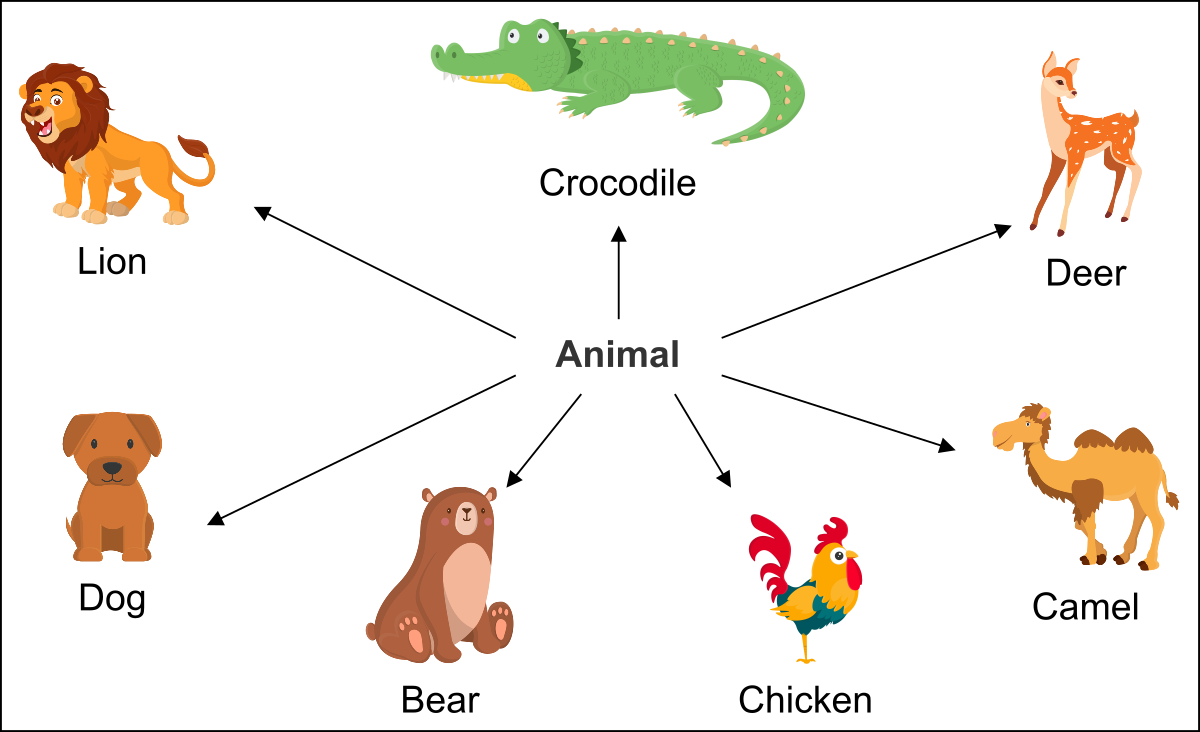
\includegraphics[width=0.5\textwidth]{Images/chapter_2/section_4612292360798208/6207528637825024.png}
 \caption{The Animal class}
\end{figure}

\subsection{Types of polymorphism}\label{-yDmGhFtFlxlNVvtRihGo-1}
\\
There are two types of polymorphism: dynamic polymorphism and static polymorphism, as shown in the figure below.

\begin{center}
\fbox{\begin{minipage}{0.9\textwidth}
\centering
\vspace{0.2cm}
\textbf{\large Types of polymorphism}
\\[0.2cm]
\textit{[Interactive Mind Map - See online version for interactive visualization]}
\vspace{0.2cm}
\end{minipage}}
\end{center}

\vspace{0.3cm}
\begin{itemize}
\item \textbf{Polymorphism}
\begin{itemize}
\item \textbf{Dynamic Polymorphism}
\begin{itemize}
\item Method Overriding
\end{itemize}
\end{itemize}
\begin{itemize}
\item \textbf{Static Polymorphism}
\begin{itemize}
\item Method Overloading
\item Operator Overloading
\end{itemize}
\end{itemize}
\end{itemize}

\subsubsection{Dynamic polymorphism}\label{-yDmGhFtFlxlNVvtRihGo-2}
\\
\textbf{Dynamic} \textbf{polymorphism} is the mechanism that defines the methods with the same name, return type, and parameters in the base class and derived classes. Hence, the call to an overridden method is decided at runtime. That is why dynamic polymorphism is also known as \textbf{runtime} \textbf{polymorphism}. It is achieved by method overriding.
\\
\paragraph{Method overriding}\label{7bkY7h9LjORzm16PusD4P}
\\
In object-oriented programming, if a subclass provides a specific implementation of a method that had already been defined in one of its parent classes, it is known as \textbf{method overriding}.
\\
Suppose we have a parent class, \texttt{Animal}, with its subclass, \texttt{Lion}. Below is the implementation of two functions with the same name in each class to check method overriding behavior.

\textbf{Method overriding example}

\begin{lstlisting}[language=Java]
class Animal {
	public void printAnimal() {
		System.out.print("I am from the Animal class
");
	}
	void printAnimalTwo() {
		System.out.print("I am from the Animal class
");
	}
}

class Lion extends Animal {
	// method overriding
	public void printAnimal() {
		System.out.print("I am from the Lion class
");
	}
}

public class main {
	public static void main(String[] args) {
		Animal animal;
		Lion lion = new Lion();
		animal = lion;

		animal.printAnimal();
		animal.printAnimalTwo();
	}
}
\end{lstlisting}

\subsubsection{Static polymorphism}\label{-yDmGhFtFlxlNVvtRihGo-3}
\\
\textbf{Static} \textbf{polymorphism} is also known as compile-time polymorphism, and it is achieved by method overloading or operator overloading.
\\
\paragraph{Method overloading}\label{aamyixSY_rP2wA5BBijn9}
\\
Methods are said to be \textbf{overloaded} if a class has more than one method with the same name, but either the number of arguments is different, or the type of arguments is different. We have implemented method overloading using two functions with the same name but with different numbers of arguments. You can see this in the implementation below.

\textbf{Method overloading example}

\begin{lstlisting}[language=Java]
class Sum {

  public int addition(int a, int b) {

	  return a + b;

  }



  public int addition(int a, int b, int c) {

	  return a + b + c;

  }

}



public class main {

  public static void main(String[] args) {

    Sum sum = new Sum();

	System.out.print(sum.addition(14, 35));

	System.out.print("
");

	System.out.print(sum.addition(31, 34, 43));

  }

}
\end{lstlisting}

\textbf{Method overloading example}

\begin{lstlisting}[language=Java]
class Area {

  public double calculateArea(double length, double breadth) {

    return length * breadth;

  }



  public double calculateArea(double side) {

	  return side * side;

  }

}



public class main {

  public static void main(String[] args) {

    Area area = new Area();

    System.out.print("Area of rectangle = " + area.calculateArea(3, 4));

    System.out.print("
");

    System.out.print("Area of square = " + area.calculateArea(6));

  }

}
\end{lstlisting}

\paragraph{Operator overloading}\label{-yDmGhFtFlxlNVvtRihGo-4}
\\
\textbf{Operators} can be overloaded to operate in a certain user-defined way. Its corresponding method is invoked to perform its predefined function whenever an operator is used. For example, when the \texttt{+} operator is called, it invokes the special function, \texttt{add}, but this operator acts differently for different data types. The \texttt{+} operator adds the numbers when it is used between two \texttt{int} data types and merges two strings when used between \texttt{string} data types.
\\
Let's look at the implementation below, where we've overloaded the \texttt{+} operator to add complex numbers instead of simply adding two real numbers.

\textbf{Operator overloading example}

\begin{lstlisting}[language=C]
using System;

class ComplexNumber {
    float real;
    float imaginary;
    // Constructor
    public ComplexNumber(float real, float imaginary) {
      this.real = real;
      this.imaginary = imaginary;
    }
    
    public override string ToString() {
        return(String.Format("( {0} + {1} i )", real, imaginary));
    }
    
    // Overloading function for + 
    public static ComplexNumber operator+(ComplexNumber c1, ComplexNumber c2) {
        return(new ComplexNumber(c1.real + c2.real, c1.imaginary + c2.imaginary));
    }
}

class MainClass {
    public static void Main() {
        ComplexNumber c1 = new ComplexNumber(11, 5);
        ComplexNumber c2 = new ComplexNumber(2, 6);
        ComplexNumber c3 = c1 + c2;
        // display results
        Console.WriteLine(c3);
    }
}
\end{lstlisting}

\begin{quote}
\textbf{Note:} Java and JavaScript do not support operator overloading.
\end{quote}
\subsubsection{Dynamic polymorphism vs. static polymorphism}\label{XwZUC079mTL3lA1hk_EuY}
\\
The table below provides a highlight of the differences between dynamic and static polymorphism:

\begin{table}[htbp]
\centering
\small
\adjustbox{max width=\textwidth}{
\begin{tabular}{|p{0.474\textwidth}|p{0.476\textwidth}|}
\hline
\textbf{Static Polymorphism} & \textbf{Dynamic Polymorphism} \\
\hline
\hline
Polymorphism that is resolved during compile-time is known as static polymorphism. & Polymorphism that is resolved during runtime is known as dynamic polymorphism. \\
\hline
Method overloading is used in static polymorphism. & Method overriding is used in dynamic polymorphism. \\
\hline
Mostly used to increase the readability of the code. & Mostly used to have a separate implementation for a method that is already defined in the base class. \\
\hline
Arguments must be different in the case of overloading. & Arguments must be the same in the case of overriding. \\
\hline
Return type of the method does not matter. & Return type of the method must be the same. \\
\hline
Private~and~sealed~methods can be overloaded. & Private~and~sealed~methods cannot be overridden. \\
\hline
Gives better performance because the binding is being done at compile-time. & Gives worse performance because the binding is being done at runtime. \\
\hline
\end{tabular}
}
\end{table}

Let\textquotesingle s test our OOP concepts in the next lesson.

% End of section content